%\documentclass[show notes]{beamer}
%\documentclass[handout]{beamer}
\documentclass[]{beamer}

\usepackage{pgfpages}
\usepackage[utf8]{inputenc}
\usepackage[T1]{fontenc}
%\usepackage{mathabx}
%\usepackage{mathpazo}
%\usepackage{eulervm}
%\usepackage{natbib}
\usepackage{adjustbox}
\usepackage{booktabs}
%\usepackage{svg}
\usepackage{colortbl}
\usepackage{hyperref}
\hypersetup{colorlinks=true, urlcolor=uog, linkcolor=uog, citecolor=uog}

\usepackage[backend=biber, style=authoryear, maxbibnames=99, dashed=false]{biblatex}
\addbibresource{tagged-SWCD2021.bib}


\usepackage{caption}
\captionsetup[figure]{labelformat=empty}% redefines the caption setup of the figures environment in the beamer class.


\usetheme{Madrid}
\definecolor{uog}{rgb}{0,.5,0}
\usecolortheme[named=uog]{structure}

\mode<handout>{
	\pgfpagesuselayout{4 on 1}[letterpaper] 
	\setbeameroption{show notes}
}


% The following code uses \AtBeginSection to place a frame with the section title (\insertsectionhead) inside a beamercolorbox.
% From https://tex.stackexchange.com/questions/178800/creating-sections-each-with-title-pages-in-beamers-slides
\AtBeginSection[]{
	\begin{frame}
		\vfill
		\centering
		\begin{beamercolorbox}[sep=8pt,center,shadow=true,rounded=true]{title}
			\usebeamerfont{title}\insertsectionhead\par%
		\end{beamercolorbox}
		\vfill
	\end{frame}
}

\title[Invasive Species Issues on Guam]{Overview of Invasive Species Issues on Guam}

\author[]{
	Glenn Dulla\textsuperscript{1}, Roland Quitugua\textsuperscript{2} and Aubrey Moore\textsuperscript{2}\\
	\bigskip 
	\tiny{\textsuperscript{1}Guam Department of Agriculture,
    \textsuperscript{2}University of Guam}
}

%\institute[]{College of Natural and Applied Sciences\\University of Guam}

%\titlegraphic{\includegraphics[width=2cm]{big_g2.pdf}}

\date[]{Pacific Ecological Security Conference\\Palau, October 6, 2022\\ \tiny\url{https://github.com/aubreymoore/PESC-OIA-overview/raw/main/guam-overview.pdf}}

\begin{document}
	
%\begin{frame}
    \maketitle
%\end{frame}

\begin{frame}{Hafa Adai}
	\adjincludegraphics[height=1.05\textheight,center]{images/Guam.jpg}
\end{frame}

\begin{frame}{How bad is Guam's invasive species problem?}
	\begin{itemize}
		\item Guam has 33 species listed in \textbf{100 of the World's Worst Invasive Species}
		\item Guam has 5 species listed in the \textbf{Top 10 World's Most Costly Invasive Species}.
		\item Guam's natural ecosystems, especially Guam's forests, are rapidly being destroyed by invasive species.
	\end{itemize}	
\end{frame}

\begin{frame}{How bad is Guam's invasive species problem?}
% TODO: \usepackage{graphicx} required
\begin{figure}
	\centering
	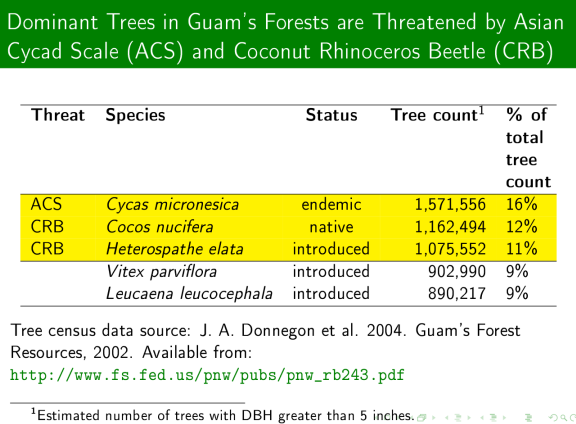
\includegraphics[width=1\linewidth]{images/dominant_trees}
	\caption{}
	\label{fig:dominanttrees}
\end{figure}
\end{frame}


\begin{frame}{Priority Issue 1: Brown treesnake}
	\adjincludegraphics[height=0.85\textheight,center]{images/bts.jpg}
	\tiny{Courtesy of USGS}
\end{frame}

\begin{frame}{Forest Birds before BTS}
	\begin{figure}
		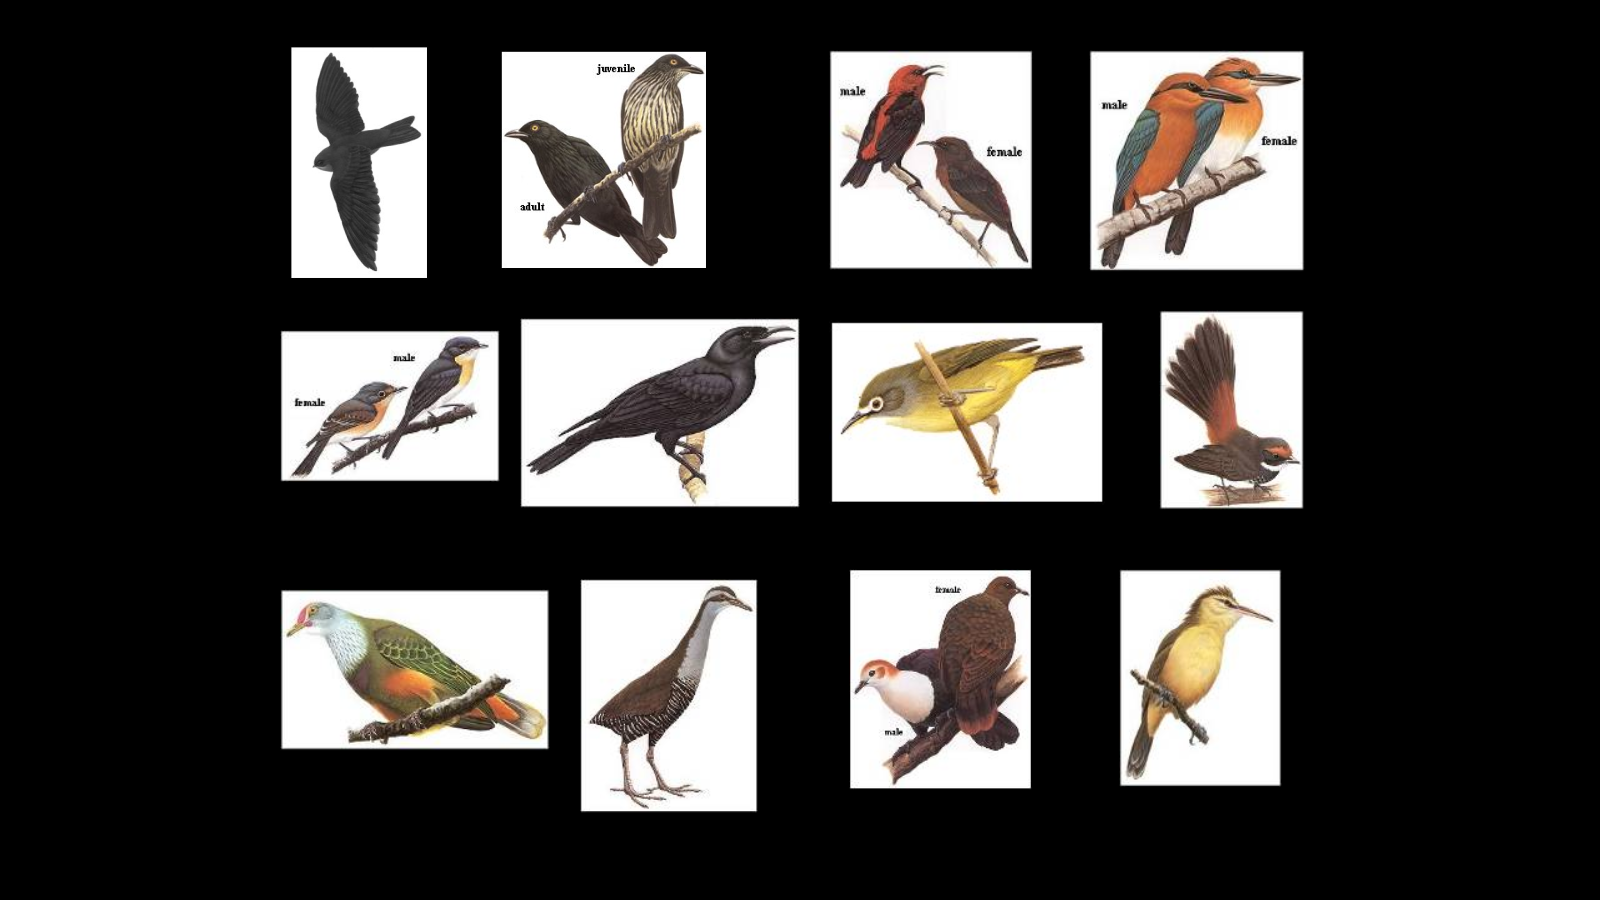
\includegraphics[height=0.8\textheight]{images/birds-before-bts.png}
	\end{figure}
\end{frame}

\begin{frame}{Forest Birds after BTS}
	\begin{figure}
		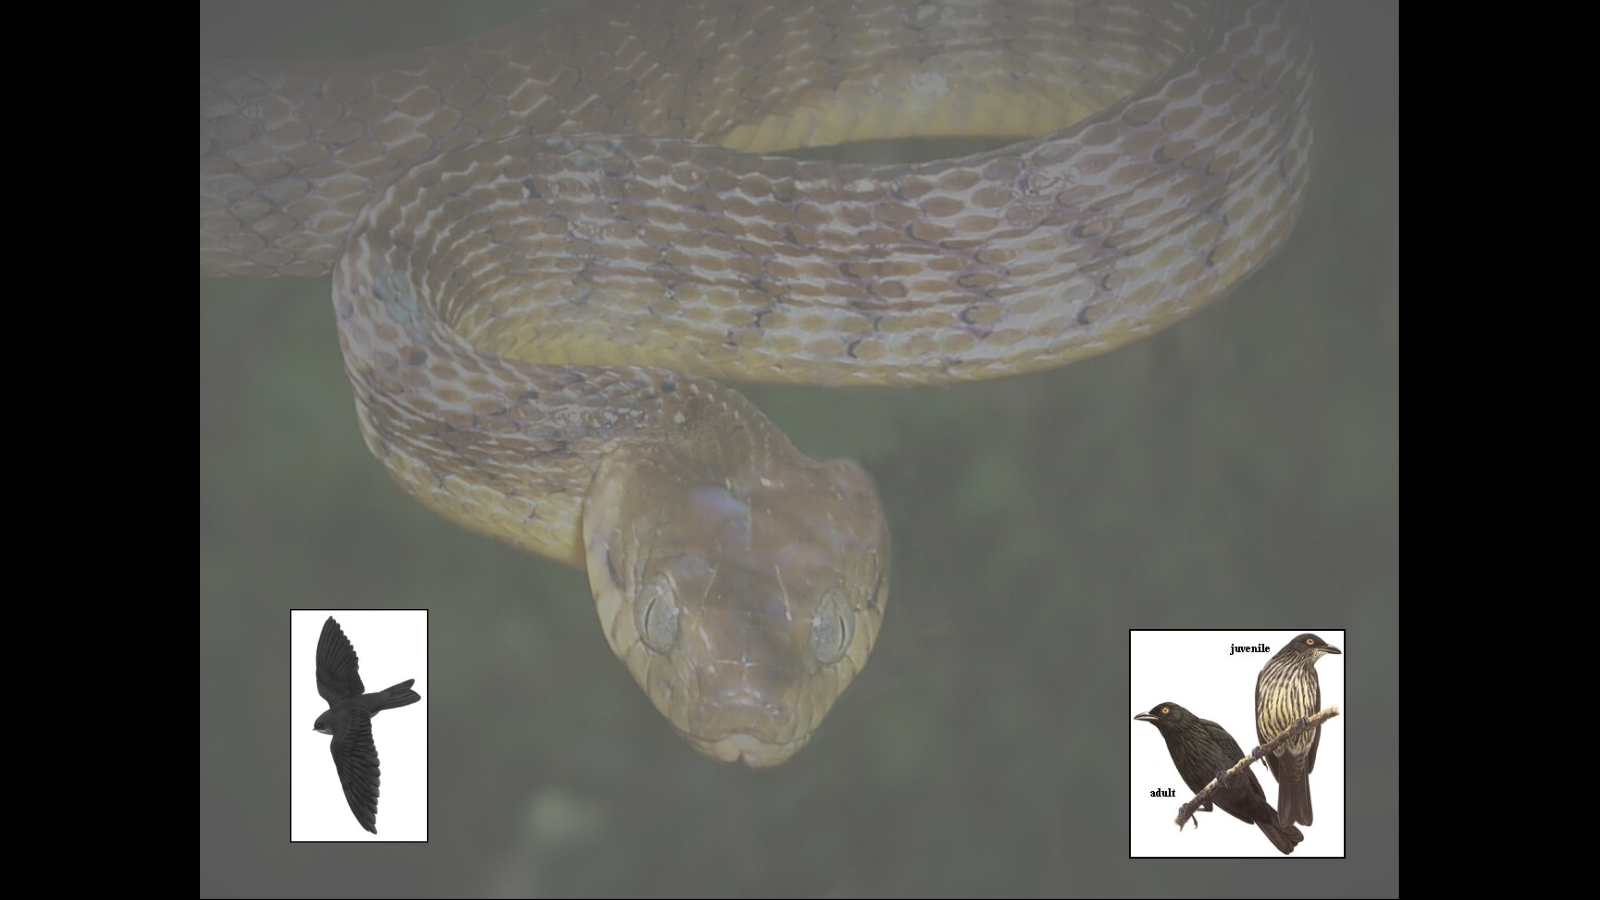
\includegraphics[height=0.8\textheight]{images/birds-after-bts.png}
	\end{figure}
\end{frame}

\begin{frame}{Priority Issue 1: Brown treesnake - Impacts}
	\begin{itemize}
		\item Following predation by BTS, Guam's forest bird species are either extinct or on the endangered species list.
		\item Forest health is severely impacted by the ecosystem services that these birds provided: seed dispersal, insect control, pollination, etc.
		\item Restoration of Guam's avifauna is unlikely without control of BTS populations. 
	\end{itemize}	
\end{frame}

\begin{frame}{Priority Issue 1: Brown treesnake - Current status}
\begin{itemize}
	\item Arrived on Guam in the late 1940s.
	\item Guam is the only place in the world where BTS has established as an invasive species
	\item Millions of dollars per year are spent on preventing BTS from leaving Guam.
	\item Some funds are being used for control methods development: snake-proof barriers and "pinkies on parachutes".
	\item Attempts at eradicating BTS from Cocos Island have not yet succeeded.
\end{itemize}	
\end{frame}

\begin{frame}{Priority Issue 2: Asian Cycad Scale}
	\adjincludegraphics[width=\textwidth]{images/output-07.png}
\end{frame}

\begin{frame}{Priority Issue 2: Asian Cycad Scale}
	\adjincludegraphics[width=\textwidth]{images/output-19.png}
\end{frame}

\begin{frame}{Priority Issue 2: Cycad aulacaspis scale - Impacts}
	\begin{itemize}
		\item Cycad aulacaspis scale, and other invasive species, have killed about 90\% of Guam's endemic \textit{Cycas micronesica} plants and the population is not recovering because natural reproduction is not occurring.
		\item{\textit{C. micronesica} went from being the most numerous tree in Guam's forests in 2002 to being placed on the National Endangered Species list in 2016}
	\end{itemize}
\end{frame}

\begin{frame}{Priority Issue 2: Cycad aulacaspis scale - Current status}
\begin{itemize}
	\item Detected on Guam in 2003; Also in Hawaii, Guam, CNMI, Palau; Endemic cycad population on Yap at great risk.
	\item Cycad aulacaspis scale is partially controlled by introduced predators and parasites on Guam, but almost all seeds and seedlings are being killed by the scale insect.
\end{itemize}	
\end{frame}

\begin{frame}{Priority Issue 3: Coconut rhinoceros beetle}
	\adjincludegraphics[width=\textwidth]{images/eve.png}
\end{frame}

\begin{frame}{Priority Issue 3: Coconut rhinoceros beetle - Impacts}
	\begin{center}
		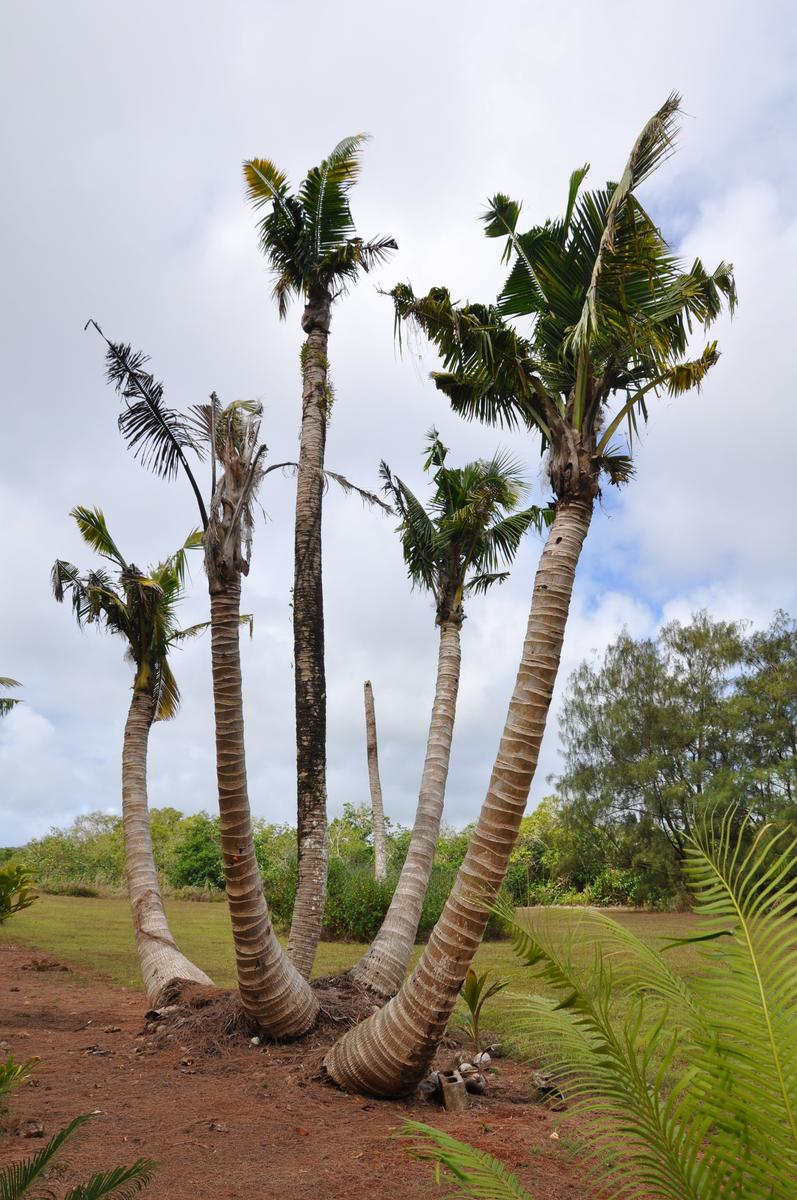
\includegraphics[height=\textheight]{images/dying_coconuts}
	\end{center}
\end{frame}

\begin{frame}{Priority Issue 3: Coconut rhinoceros beetle - Impacts}
	\begin{itemize}
		\item A severe, uncontrolled outbreak of coconut rhinoceros beetle (CRB) on Guam is damaging and killing coconut palms and other palms. \item Island-wide, roadside damage surveys indicate that about 20\% of coconut palms show visible CRB damage.
		\item  Pheromone trap data and damage surveys have shown no significant upward or downward trend in the past 2 years and trees continue to be killed.
	\end{itemize}
\end{frame}

\begin{frame}{Priority Issue 3: Coconut rhinoceros beetle - Current status}
	\begin{itemize}
		\item First detected on Guam in 2007; also established in American Samoa, Palau, Guam, Hawaii (Oahu), and the CNMI (Rota)
		\item Palau, Guam, Hawaii, and CNMI have a virus-resistant strain, CRB-G, which does not respond to \textit{Oryctes rhinoceros} nudivirus which was previously a highly effective self-sustaining biological control agent
		\item Much of the current effort on Guam is directed at reducing risk of accidental exporting CRB by attempts to reduce populations in proximity of ports and to increase outgoing biosecurity 
		\item CRB-G is killing coconut palms throughout Guam. In some areas coconut palm mortality is almost 100\%
	\end{itemize}
\end{frame}

\begin{frame}{Priority Issue 4: Little fire ant}	
	\begin{figure}
	\adjincludegraphics[width=\textwidth]{images/lfa-pencil.jpg}
	\end{figure}
\end{frame}

\begin{frame}{Priority Issue 4: Little fire ant - Impacts}	
	\begin{itemize}
		\item \textbf{Human health.} LFA stings cause painful welts and produce varying allergic reactions. 
		\item \textbf{Animal health.} stings to animal eyes cause a clouding or keratopathy leading to blindness
		\item \textbf{Ecological impacts.} LFA is highly competitive and displaces other invertebrates and vertebrates in infested areas. Mutualisms between LFA and Hemiptera causes explosions of plant pests, dramatically decreasing plant health and productivity.
		\item \textbf{Economic impacts.} Heavily infested structures and properties become uninhabitable without treatment. Guam's tourist industry is expected to be impacted.				
	\end{itemize}
\end{frame}

\begin{frame}{Priority Issue 4: Little fire ant - Current status}	
	\begin{itemize}
		\item First detected on Guam in 2011. Also in Hawaii and Yap (FSM)
		\item LFA has been documented to be in every village on Guam
		\item LFA identified at Guam ports, some in critical loading  areas with direct transport to neighboring islands
%		\item Availability of pesticides remain limited and preferred chemicals can be cost prohibited
%		\item Spread of LFA enhanced by lack of public green waste management system
%		\item Current ecological studies on Guam are measuring LFA impacts on invertebrate diversity on conservation and public lands
%		\item Social and economic impact are present on Guam, but are not being tracked or quantified in any meaningful way
%		\item Short-term federal funding cover focused management in conservation areas and ports
%		\item Almost no funding input from local government
	\end{itemize}
\end{frame}

\begin{frame}{Challenges}
	Human Resources
	\begin{itemize}
		\item Professional scientific/technical capacity is low
		\item Guam suffers from the \textit{taxonomic impediment}
		\item Guam does not have a terrestrial biodiversity inventory
	\end{itemize}
	Funding
	\begin{itemize}
		\item Invasive species projects on Guam are funded by many relatively small short-term competitive grants. Project management overhead (proposal writing and report writing) is very high, leaving little time to actually do the work.
	\end{itemize}
\end{frame}

\begin{frame}{Funding sources}
	\begin{itemize}
	   \item Department of Interior - Office of Insular Affairs
	   \item USDA - Forest Service
	   \item USDA - APHIS
	   \item DOD
	   \item Government of Guam - Invasive Species Tarrif
	\end{itemize}		
\end{frame}

\begin{frame}{National/Territorial Invasive Species Plans}
	\begin{itemize}
		\item Guam Invasive Species Management Plan \url{https://www.sprep.org/attachments/VirLib/Guam/nissap-2017-2019.pdf}
		\item Regional Biosecurity Plan for Micronesia and Hawaii
		\url{https://pacific.navfac.navy.mil/About-Us/Regional-Biosecurity-Plan-for-Micronesia-and-Hawaii/}
	\end{itemize}	
\end{frame}

\begin{frame}{Next steps}
	\textbf{Find and implement solutions for priority issues}
	\begin{itemize}
%		\item Update and implement action items in the \textbf{Guam Invasive Species Management Plan} and the \textbf{Regional Biosecurity Plan for Micronesia and Hawaii}
		\item \textbf{Brown treesnake.} Eradicate BTS from Cocos Island
		\item \textbf{Cycad aulacaspis scale.} Implement an effective, island-wide, self-sustaining biocontrol program which will allow natural reproduction of surviving cycads (as per recommendations by Dr. Ronald Cave \url{https://github.com/aubreymoore/CAS-biocontrol-seminar/raw/main/Cave-CAS-report-2022.pdf})
		\item \textbf{Coconut rhinoceros beetle.} Implement an effective, island-wide, self-sustaining biological control program for CRB-G which will suppress populations, reduce damage and halt palm mortality.
		\item \textbf{Little fire ant.} Continue local outreach to slow spread; population control around ports, conservation areas, and beach parks; evaluation of biocontrol agents
	\end{itemize}

\end{frame}

\begin{frame}{The End - Thanks for listening.}
	\adjincludegraphics[width=\textwidth]{images/output-53.png}
\end{frame}


\end{document}
